\headline{{\textbf{\Large\sffamily Bonsai Roots:}}\\
          {\textbf{\large\sffamily Meet the Members of TWBC}}}
\label{2025-06-roots}
\noindent
In every edition of \emph{Bonsai Roots,} we step away from wiring and watering for a moment to celebrate the members who make our club so special.
Everyone's story adds a new leaf to the rich tapestry of TWBC.
This month, we're excited to introduce \textbf{Riz Mirza!}

\begin{itemize} 
    \item \textbf{What's your name and where in the country do you live?}

    \emph{I'm Riz Mirza, and I live in Ham, near Kingston.}

    \item \textbf{What are your favourite species of tree and why?}

    \emph{Although I have a fondness for all species, I'm particularly drawn to Maples and Redwoods. That said, I have a real soft spot for our native trees, especially Larch and Yew.}

    \item \textbf{What aspect of bonsai do you enjoy?}

    \emph{I'm still very much a novice, but I'm loving the learning process --- especially getting hands\--on. Honestly, just seeing a tree survive feels like a big win!}

    \item \textbf{What aspects of bonsai do you find most challenging?}

    \emph{Probably branch selection. Decisions, decisions\dots}

    \begin{window}[%
        2,l,%
        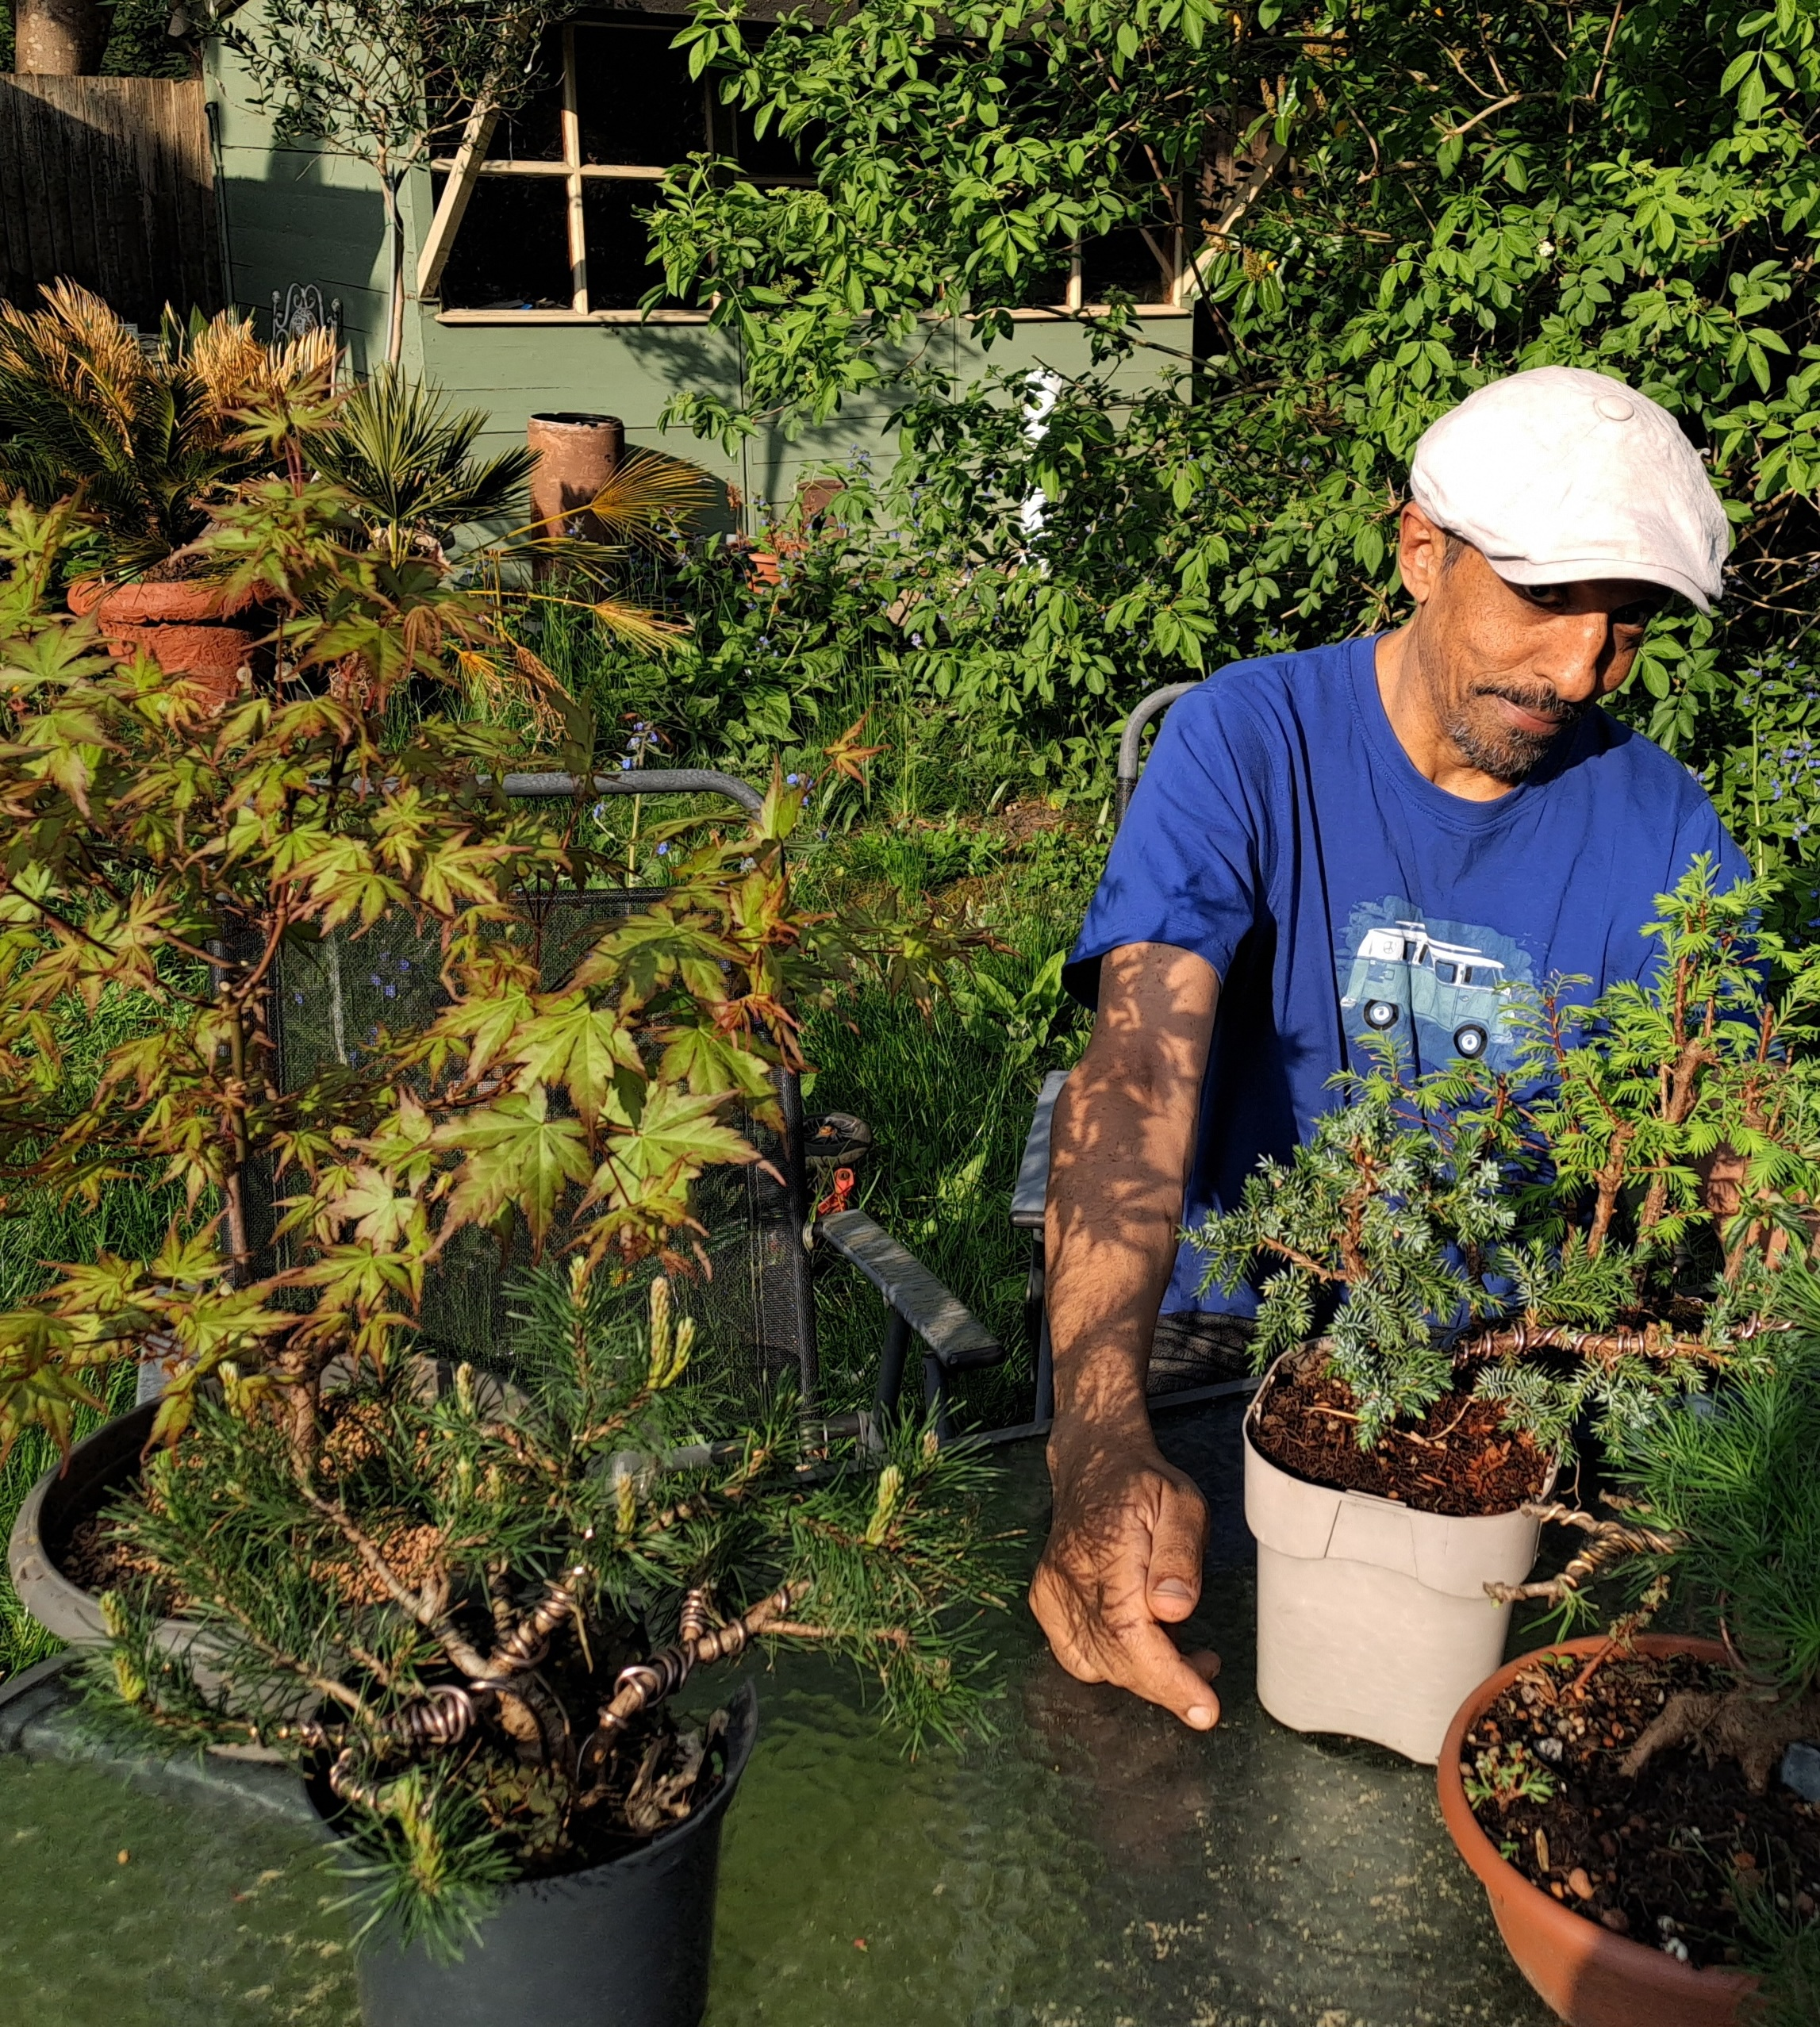
\includegraphics[width=1.0\columnwidth]{2025_06/res/roots_riz_mirza},%
        \centerline{\emph{Riz tending to his bonsai with patience, joy, and sunshine.}}%
    ]
    \end{window}
    \columnbreak

    \item \textbf{Who or what inspires you throughout your bonsai journey?}

    \emph{I find inspiration in the process itself --- just being in the moment with the trees. Seeing the amazing work of others definitely keeps me motivated too.}
    
    \item \textbf{How long have you been interested in keeping bonsai?}

    \emph{Ooh, for quite some time now. I've always enjoyed the challenge of growing exotic plants like bananas, palms, and cannas --- and from there, bonsai naturally caught my interest. I joined another club before but found it a bit too restrictive.}

    \item \textbf{What stimulated your interest in bonsai?}

    \emph{The natural beauty of plants --- it's as simple and as powerful as that.}

    \item \textbf{If you could give someone new to bonsai any tips, what would it be?}

    \emph{Join Twickenham Bonsai! And just trust yourself --- it's all part of learning. Remember, it's a journey, not a destination.}

    \item \textbf{Why do you enjoy being part of TWBC, and do you have any ideas or suggestions for the club's future?}

    \emph{The friendly, open atmosphere is brilliant. There's so much encouragement, expert advice, and plenty of good banter. I met Tony at an event, and within five minutes of arriving at a meeting, I knew this was the place for me.}

    \item \textbf{One word to describe what bonsai means to you?}

    \emph{Yew!}

    \item \textbf{What are your future goals regarding your own trees and learning more about the hobby?}

    \emph{Just to keep enjoying it! I want to attend more workshops, get along to events, tap into everyone's experience, and read different books to keep learning.}

    \item \textbf{How would you like to see your bonsai journey progress in the future?}

    \emph{I'm aiming to enjoy every step of the process, with no pressure --- just a love for the trees.}
\end{itemize}

It's been brilliant to hear about Riz's bonsai story --- full of good humour and a real love for the craft.
Who will we get to know next time? Stay tuned for more in \emph{Bonsai Roots}!

\begin{center}
    $\cdots$
\end{center}

\noindent
\emph{If you're a newer member and would like to feature in a future edition of Bonsai Roots, simply fill out the form at \href{https://forms.gle/quVXa4L8rhpnT5kr6}{this link}! We'd love to hear your story.}
\closearticle 
\pagebreak
